% Nejprve uvedeme tridu dokumentu s volbami
\documentclass[czech,master]{diploma}
% Dalsi doplnujici baliky maker
\usepackage[autostyle=true,czech=quotes]{csquotes} % korektni sazba uvozovek, podpora pro balik biblatex
\usepackage[backend=biber, style=iso-numeric, alldates=iso]{biblatex} % bibliografie
\usepackage{dcolumn} % sloupce tabulky s ciselnymi hodnotami
\usepackage{subfig} % makra pro "podobrazky" a "podtabulky"
\usepackage[cpp]{diplomalst}

% Zadame pozadovane vstupy pro generovani titulnich stran.
\ThesisAuthor{Bc. Marek Lukáš}

\ThesisSupervisor{Ing. David Seidl, Ph.D.}

\CzechThesisTitle{Eink display jako informační panel}

\EnglishThesisTitle{Eink Display on Information Panel}

\SubmissionYear{2024}

\ThesisAssignmentFileName{Zadani.pdf}

% Pokud nechceme nikomu dekovat makro zapoznamkujeme.
\Acknowledgement{TODO}

\CzechAbstract{TODO}

\CzechKeywords{esp32, inkplate, eink}

\EnglishAbstract{TODO}

\EnglishKeywords{esp32, inkplate, eink}

% bibliografie
\addbibresource{bibliography.bib}

% zkratky
\AddAcronym{SoC}{System on chip, systém zahrnující všechny komponenty počítače v jediném čipu}
\AddAcronym{UART}{Universal asynchronous receiver-transmitter}
\AddAcronym{EPD}{Electronic paper display}
\AddAcronym{API}{Application programming interface}
\AddAcronym{SDK}{Software development kit}
\AddAcronym{RTTI}{Runtime type information}
\AddAcronym{HAL}{Hardwer abstraction layer}
\AddAcronym{LL}{Low level layer}
\AddAcronym{RTC}{Real time clock}
\AddAcronym{e-ink}{Elektronický inkoust}
\AddAcronym{IDE}{Integrated Development Environment}
\AddAcronym{IoT}{Internet of Things, internet věcí}

% Novy druh tabulkoveho sloupce, ve kterem jsou cisla zarovnana podle desetinne carky
\newcolumntype{d}[1]{D{,}{,}{#1}}


% Zacatek dokumentu
\begin{document}

% Nechame vysazet titulni strany.
\MakeTitlePages

% Jsou v praci obrazky? Pokud ano vysazime jejich seznam a odstrankujeme.
% Pokud ne smazeme nasledujici dve makra.
\listoffigures
\clearpage

% Jsou v praci tabulky? Pokud ano vysazime jejich seznam a odstrankujeme.
% Pokud ne smazeme nasledujici dve makra.
\listoftables
\clearpage

% A nasleduje text zaverecne prace.
\chapter{Úvod}

Elektronické inkoustové panely, známé také jako e-ink displeje, představují revoluční technologii zobrazování informací, která nachází uplatnění v širokém spektru aplikací od čteček elektronických knih až po informační tabule. Naše fakulta se rozhodla využít tuto technologii k zefektivnění komunikace uvnitř budovy. Cílem tohoto projektu je vytvořit systém, který umožní dynamické zobrazování obsahu na e-ink displejích prostřednictvím WiFi, čímž se sníží potřeba manuální aktualizace a zvýší se efektivita správy fakultních prostor. Implementace tohoto systému umožní flexibilní a okamžité šíření informací spjatých se strategickými místy fakulty.

Prvním z cílových míst jsou zasedací místnosti, u kterých je běžné, že se průběžně mění rozpis jejich rezervací. Bez denně aktualizované tabulky rozpisu nelze jednoduše zjistit, jaká schůzka se právě koná a kdy bude místnost opět volná. S elektronickým panelem lze rozpis automaticky aktualizovat a mít tak vždy aktuální přehled o plánu místnosti.

Přednáškové místnosti jsou dalším z míst, kde je záhodno mít možnost dynamického rozvrhu. Z technických důvodů mohou být přednášky přesunuty do jiné místnosti nebo se může konat mimořádná přednáška mimo pravidelný rozvrh. Panely ale nemusí sloužit jen pro účely rozvrhu. Mohou ukazovat čas, pokyny od pedagogů, promo obsah, fotky nebo akutní varování.

Práce je rozdělena do pěti základních kapitol. První kapitola popisuje hardware a prostředí, pro které je systém určen. Zaměřena je především na popis samotných panelů, na kterých je tato práce postavena. Je zmíněna jejich softwarová a hardwarová architektura, možnosti, které nabízejí a limitace, se kterými bylo nutno pracovat při vývoji a návrhu. Zahrnuta je také analýza technologie elektronického inkoustu, jeho výhod, omezení v kontextu tohoto projektu.

Druhá kapitola se zaměřuje na systém jako celek. Prochází historii návrhu systému a zmiňuje slepé uličky, které tvarovaly podobu konečného systému. Finálem kapitoly je popis stávající architektury systému. Kapitola slouží jako základ ke snadnějšímu porozumění následujících kapitol o jednotlivých částech systému. Důraz je kladen na modulární design a flexibilitu systému, které umožňují snadnou adaptabilitu na měnící se požadavky a integraci nových funkcionalit.

Třetí kapitola se věnuje samotné implementaci jednotlivých částí navrženého systému. Každá její část obsahuje popis implementovaných API. Od návrhu po jejich implementaci. V první části kapitoly je popsána implementace firmwaru panelu. V další je popsán backend systému. Třetí část se zabývá implementací webové aplikace sloužící k autentizované interakci s jednotlivými komponentami. Rozbor každé části zahrnuje technické detaily a výzvy, se kterými jsem se setkal, a způsoby, jakými jakými jsem se rozhodl výzvy řešit.

Čtvrtá kapitola popisuje, jak byl systém nasazen v produkčním prostředí a jaké technologie jsou použity pro jeho sestavení a údržbu. Tato část završuje celý proces vývoje.

V poslední kapitole navrhuji možné budoucí úpravy a vylepšení, které byly, z různých důvodů, vypuštěny z finálního návrhu. Diskutovány jsou i strategie pro zajištění standardu bezpečnosti pro možnost nasazení mezi široký okruh uživatelů. Jde o důležitou kapitolu pro navazující práce, které by rozšiřovaly tento systém.

\chapter{Hardware a prostředí}

\section{Inkplate 10}
Středem celého projektu je panel Inkplate 10 od chorvatské společnosti Soldered Electronics. Ta jej uvedla na trh začátkem roku 2021, ještě pod svým tehdejším jménem e-radionica \cite{solderedelectronicsUs}, na crowdfundingové platformě Crowd Supply \cite{zovkoOurCampaignLive2021}.
Kampaň měla za cíl vybrat 12 900 \$. To se podařilo za méně než 24 hodin \cite{crowdsupplyna[@crowd_supply]NewCampaignLaunched2021} a ve výsledku e-radionica vybrala přes 178 tisíc dolarů \cite{solderedelectronicsInkplate102021}.

Panel disponuje 9,7 palcovým e-ink displejem o rozlišení 1200 na 825 pixelů, USB-C portem, třemi kapacitními tlačítky, a integrovaným čipem ESP32.

Oproti jiným panelům, jako jsou např. Waveshare EPD a Adafrui EPD, lze Inkplate 10 používat bez dodatečného hardwaru. Kromě samotného e-ink displeje je na jeho desce zabudovaný i modul mikrokontroleru ESP32-WROVER. Díky němu lze do Inkplatu snadno nahrát vlastní firmware a zobrazit například fotky ze zabudované čtečky MicroSD karet či z internetu přes zabudovanou Wi-Fi anténu \cite{solderedelectronicsInkplate102021}.

\section{Možnosti zobrazení a omezení}

Displej funguje na technologii elektronického inkoustu a pochází z vyřazených zařízení několika výrobců. Mezi hlavní zdroje patří čtečky Amazon Kindle \cite{solderedelectronicsInkplate102021}. Obraz na panelu zůstává a je vidět i po odebrání napájení. Díky tomu je při málo frekventovaných aktualizacích vysoce úsporný. V případě mikrokontroleru stačí systém probudit z hlubokého spánku, např. jen jednou za minutu, zjistit požadovaný stav, překreslit displej a na celou následující minutu se znovu uspat. Displej zůstane nadále čitelný \cite{heikenfeldReviewPaperCritical2011}.

Každý pixel přitom může nabývat až 8 odstínů šedi, tedy 3 bity na jeden pixel. Aktualizace obrazu v tomto režimu trvá, dle výrobce, 1,81 sekundy.
V černobílém režimu (režim 1 bit na pixel) podporuje i částečné překreslení, které zvládá za 0,62 sekundy \cite{solderedelectronicsInkplate102021}. Při mém testování byly tyto časy ale o něco delší.

Důvodem pro relativně dlouhý čas pro překreslení panelu je technologie e-ink, tedy elektronický inkoust. Technologie (černo-bílého e-inkoustu) funguje na bázi fyzických miniaturních mikrokapslí, zhruba o průměru lidského vlasu. Každá kapsle obsahuje kladně nabité bílé částice a záporně nabité černé částice zachycené v čiré kapalině. Podle polarity elektrického pole v kapsli se černé a bílé částice rozdělí ke korespondujícím elektrodám u povrchu, čímž se daná kapsle zbarví do bíla či černa \cite{einkholdingsinc.ElectronicInkInk}. V případě panelů podporujících odstíny šedi, nejsou částice přesunuty plně k povrchu, ale jen částečně tak, aby poměr bílých a černých částic u povrchu na pohled připomínal cílený odstín šedi \cite{adafruitindustriesTHINKINKHow2020}. Jsou k tomu použity velmi přesné střídavé náboje. Pomalé vykreslování je způsobené relativně dlouhou dobou nutnou k přesunu částic a jejich ustálením. Navíc přesun částic není plně spolehlivý a při vykreslování je běžné, že některé skupiny částic zůstanou nepřesunuté, e-ink displeje bývá nutno relativně často resetovat cyklickým překreslením černého a bílého stavu \cite{heikenfeldReviewPaperCritical2011}.

\section{Programování Inkplate}

Pro účely programování nabízí Inkplate:
\begin{itemize}
    \item dvoujádrový procesor s frekvencí až 240 MHZ
    \item 8 MB paměti RAM
    \item 4 MB paměti flash
    \item USB-C port
    \item integrovanou podporu Wi-Fi a Bluetooth 4.0 \cite{solderedelectronicsInkplate102021}
    \item integrovaný USB-UART konvertor
    \item integrovaný časovač (RTC) \cite{solderedelectronicsInkplateFeaturesInkplate}
    \item volně přístupné GPIO piny s nativní podporou protokolů I\textsuperscript{2}C, SPI a easyC/Qwiic
\end{itemize}

\subsection{ESP32}
Zabudovaný mikrokontroler je založený na čipu ze série ESP32 od čínské společnosti Espressif Systems \cite{espressifEspressifEspressifSystems}. Jedná se o nástupce čipu ESP8266 z roku 2014. ESP32 bylo uvedeno o dva roky později v září 2016 \cite{espressifEspressifAnnouncesLaunch}. Čip je známý svou relativně nízkou cenou, integrovanou konektivitou, vysokým výkonem a otevřeností svého firmwaru. Staví se mezi nejčastěji používané mikrokontrolery na světě\cite{espressifEspressifLeadsIoT}\cite{espressifEspressifEspressifSystems}.

Byl navržen pro mobilní zařízení, průmyslovou automatizaci a internet věcí. Pro účely omezení spotřeby energie nabízí několik režimů spánku, dynamické škálování výkonu a relativně nízkou aktivní spotřebu hlavního procesoru. V režimu hlubokého spánku jeho spotřeba padne až na $10 \mu A$ i při zachování napájení RTC paměti. Pro aplikace kritické na bezpečnost nabídne hardwarově akcelerované kryptografické šifry, Secure Boot (ověření podpisu zaváděného firmwaru) a obecné šifrování flash paměti \cite{esp32_datasheet}. 

Všechny čipy ESP32 nabízí\cite{espressifProductOverviewESP32}:
\begin{itemize}
    \item Wi-Fi (2,4 GHz)
    \item Bluetooth 4.0
    \item dvoujádrový 32-bitový procesor Tensilica Xtensa LX6 operujiící až na 240 MHz
    \item ULP koprocesor\cite{ULPCoprocessorProgramming}
\end{itemize}

\subsection{ESP-IDF}
Oficiální vývojové prostředí pro čipy řady ESP. Bylo vyvíjeno otevřeně pod open-source licencí Apache License 2.0 od uvedení ESP32 \cite{grokhotkovInitialPublicVersion2016}. ESP-IDF je založeno na implementaci operačního systému FreeRTOS, ale nabízí i ucházející podporu API kompatibilních se standardem POSIX. Pro příklad lze pro tvorbu vláken používat jak nativní \lstinline|xTaskCreate| z FreeRTOS tak i posixové \lstinline|pthread_create| \cite{espressifPOSIXThreadsSupport}. Zdrojový kód projektů závisejících na ESP-IDF se díky tomu téměř neliší od projektů pro běžné posixové operační systémy.

Od verze v2.0 podporuje projekty využívající C++ a STL \cite{grokhotkovReleaseESPIDFRelease} a ve své aktuální verzi v5.2 podporuje standard C++23. S omezeními zvládá podporu C++ vláken, mutex, výjimek i RTTI \cite{espressifSupportESP32ESPIDF}. Vlákna a mutex jsou postavené nad interní implementací \lstinline|pthread.h| \cite{espressifPOSIXThreadsSupport}.

Kromě standardní knihovny C/C++ obsahuje SDK funkce pro přístup k hardwaru čipů ESP, jako je Wi-Fi, Bluetooth, persistentní paměť, JTAG debugging, HAL a LL abstrakce, zabezpečení bootloaderu a Over-The-Air aktualizace \cite{espressifAPIGuidesESP32}.

\subsection{Oficiální knihovny}
Soldered Electronics pro své panely vyvíjí a udržuje knihovny pro dvě vývojové platformy. Arduino a MicroPython. Nabízejí jednotné API pro práci s jakýmkoliv panelem od této společnosti. Obě pokrývají všechny základní potřeby pro interakci s displejem, přístup k hardwaru specifického pro jednotlivé panely a řadu pomocných funkcí např. pro dekódování obrázků či připojení k síti Wi-Fi.

\begin{table}[h]
    \centering
    \caption{Srovnání aktivity repozitářů knihoven pro vývoj pro panely Inkplate (větev master, 02.04.2024)}
    \label{tab:inkplate-library-comparison}
    \begin{tabular}{llll}
        \multicolumn{1}{c}{}
            & Inkplate Arduino\cite{SolderedElectronicsInkplateArduinolibrary2024}
            & Inkplate MicroPython\cite{SolderedElectronicsInkplatemicropythonMicropython}
            & Inkplate ESP-IDF\cite{turcotteTurgu1ESPIDFInkPlate2024} \\ \hline
        první commit             & 15.12.2019 & 17.08.2020  & 23.12.2019 \\
        poslední commit          & 01.04.2024 & 19.02.2024  & 09.02.2023 \\
        počet commitů            & 1330       & 123         & 162        \\
        ot./uz. issues           & 3/140      & 5/15        & 5/8        \\ \hline
    \end{tabular}
\end{table}

\subsubsection{Inkplate Arduino}
Platforma Arduino se skládá z mikrokontrolerů, programovacího jazyka, vývojového prostředí (IDE) a ekosystému Arduino knihoven. Arduino vzniklo jako učební pomůcka na Ivrea Interaction Design Institute v Miláně. Mělo za cíl vytvořit prostředí a vývojové desky, se kterými mohou pracovat i studenti bez podrobných znalostí elektroniky a programování \cite{WhatArduino}. Z čistě učební pomůcky se postupem času stala univerzální vývojová platforma sjednocující vývoj pro mikrokontrolery různých výrobců, tak i vlastní mikrokontrolery Arduino používané v enterprise IoT zařízeních \cite{Arduino}. Na softwarové platformě Arduino lze od roku 2018 vyvíjet i pro mikrokontrolery série ESP32 pomocí oficiální implementace Arduino Core \cite{ReleasesEspressifArduinoesp32}. Ta je vrstvou integrující softwarová API Arduino nad ESP-IDF. Lze tak nejen používat Arduino jazyk pro vývoj na ESP32, ale i integrovat knihovny určené pro Arduino v ESP-IDF projektu \cite{espressifsystemsArduinoESPIDFComponent}.

Na této kompatibilní vrstvě je postavena knihovna Inkplate Arduino. Pro Soldered je tato knihovna vlajkovou lodí. Mezi knihovnami zmíněnými v této kapitole čítá její repozitář největšímu množství příspěvků a je mezi nimi též nejstarší (tabulka \ref{tab:inkplate-library-comparison}).

Pro Arduino existuje mnoho knihoven a návodů. Jde de facto o standard pro prototypování embedded zařízení. Na tento projekt se však příliš nehodila. Ne všechny knihovny pro ESP-IDF fungují pod Arduino Core a ne všechny Arduino knihovny fungují na ESP32. Jsem zastáncem moderních standardů C++, které nabízí ESP-IDF s relativně aktuální implementací standardu a kompilátoru. Inkplate Arduino však závisí na verzi Arduino Core, které podporuje, ještě v době psaní tohoto textu, jen staré ESP-IDF v4.4. Nikoliv aktuální verzi v5.2.

\begin{lstlisting}[label=src:arduino-hello-world,language=C++,caption={Ilustrační použití knihovny Inkplate Arduino}]
#include "Inkplate.h"

// vytvoření instance ovladače
Inkplate display(INKPLATE_1BIT);

void setup() {
    // inicializace ovladače
    display.begin();
    // vyčištění displeje a bufferu
    display.clearDisplay();
    display.display();
    // vykreslení kružnice
    display.drawCircle(600, 412, 75, BLACK)
    // vykreslení textu
    display.setTextColor(BLACK, WHITE);
    display.setCursor(587, 550);
    display.print("Hello, world!");
    // částečné překreslení obrazovky
    display.partialUpdate();
}
\end{lstlisting}

V ukázce \ref{src:arduino-hello-world} je znázorněn minimalistický program sloužící k ilustraci syntaxe knihovny Inkplate Arduino. Program nejprve inicializuje ovladač panelu a vyčistí displej a jeho buffer. Poté vykreslí černou kružnici se středem v souřadnicích x=600px, y=412px a poloměrem 75px. Pod kružnici je vykreseln text ,,Hello, world!".

\subsubsection{Inkplate MicroPython}
Druhá knihovna je určena pro firmware postavený na projektu MicroPython. Jedná se o kompilátor a běhové prostředí implementující programovací jazyk Python 3 optimalizované pro běh na mikrokontrolerech a v omezených prostředích. Snaží se být kompatibilní s běžnými desktopovými verzemi Pythonu. Nabízí tak interaktivní příkazovou řádku, správu výjimek, výpočty s libovolnou přesností, věstavěný souborový systém \cite{MicroPythonPythonMicrocontrollers}.

V čem se MicroPython razantně liší od od Arduina, je proces vývoje. V prostředí Arduino (a ESP-IDF) je vyvíjená aplikace kompilována na běžném počítači spolu s celým firmwarem určeného pro mikrokontroler. Výsledný obraz sice bývá optimálnější na využití prostředků mikrokontroleru, na druhou stranu tento přístup s sebou nese náročnější proces při testování aplikace a komplexnější soubory projektu jako celku. Po instalaci běhového prostředí MicroPythonu na ESP32, lze desku připojit k počítači a přihlásit se k interaktivní Python konzoli běžící na mikrokontroleru. Vyvíjené programy lze upravovat a spouštět z emulovaného flash úložiště \cite{MicroPythonPythonMicrocontrollers}. Na některých deskách lze interní filesystem připojit k systému jako běžnou USB klíčenku a upravovat uložené python skripty napřímo, bez potřeby kompilace, flashování a speciálních vývojových nástrojů \cite{WorkingFilesystemsMicroPython}. V případě, že mikrokontroler nepodporuje režim USB MSC, je pro kopírování souborů na desku nutno použít nástroj \lstinline|pyboard.py|, který však lze verzovat uvnitř projektu a je obsažen i v projektu Inkplate knihovny \cite{PyboardPyTool}.

Protože vyvíjená aplikace nemusí projít kompilací před jejím nahráním na desku, je kompilátor obsažen v MicroPython firmwaru. To má vliv na použitelnou velikost flash paměti pro vyvíjený program. Stejně tak tím, že je nutné skripty při načítání zpracovat a zkompilovat do Python bajtkódu, rychlost aplikací založených na běhovém prostředí MicroPython, bývá citelně nižší než jejich kompilovaná alternativa v C/C++, jako je například ESP-IDF v případě ESP32 \cite{plauskaPerformanceEvaluationMicroPython2022}.

Inkplate MicroPython je jednoduchá na používání a byl jsem s ní schopen panel velmi rychle zprovoznit. Při rešerši jsem však narazil na několik omezení, která mi ho neumožnila použít pro tento projekt.

Prvním z omezení byl výkon. Při mém testování jsem zjistil, že programu, stavějícím na MicroPythonu, trvá překreslení obrazovky zhruba dvakrát déle než projektu postaveném na ESP-IDF. 

\begin{lstlisting}[label=src:micropython-spiram-partition-table,caption={Tabulka oddílů vyčtena z MicroPython firmwaru pomocí nástroje esp32part}]
$ ./src/esp32part (\
  dd if=$HOME/Stažené/ESP32_GENERIC-SPIRAM-20240222-v1.22.2.bin \
  ibs=1 \
  skip=(math 0xc00) \
  count=(math 0x8000) | psub \
  )
32768+0 records in
64+0 records out
32768 bytes (33 kB, 32 KiB) copied, 0,00779111 s, 4,2 MB/s
# Name,               Type, SubType,  Offset,     Size,       Flags
nvs,                  data, nvs,      0x00009000, 0x00006000, 
phy_init,             data, phy,      0x0000f000, 0x00001000, 
factory,              app,  factory,  0x00010000, 0x001f0000, 
vfs,                  data, fat,      0x00200000, 0x00200000,
\end{lstlisting}

Dále chyběla oficiální podpora pro aktualizace firmwaru na dálku. MicroPython sice OTA aktualizace podporuje, ale ne ve firmwaru pro variantu ESP32 na Inkplate 10. Důvodem je, že knihovna pro ovládání displeje závisí na využití externího paměťového modulu \cite{SolderedElectronicsInkplatemicropython2024}. Ten je však podporován jen ve verzi MicroPython firmwaru, která má standardní tabulku oddílů a nepodporuje bezpečné aktualizace. Protože MicroPython tuto informaci nikde přímo nezmiňuje, musel jsem si ji ověřit vyčtením tabulky oddílů ze staženého firmwaru. Způsob, jakým jsem tabulku vyčetl a její rozdělení je vidět na ukázce \ref{src:micropython-spiram-partition-table}.

Hlavním omezením však bylo, že Inkplate MicroPython podporuje na Inkplate 10 pouze čtyři odstíny šedi, místo nativních osmi \cite{RenameINKPLATE_2BITINKPLATE_3BIT}. Nemělo smysl začínat projekt nad ekosystémem, který by nepodporoval takto specifickou funkcionalitu panelu.

\begin{lstlisting}[label=src:micropython-hello-world,language=Python,caption={Ilustrační použití knihovny Inkplate MicroPython}]
from inkplate10 import Inkplate

// vytvoření instance ovladače
display = Inkplate(Inkplate.INKPLATE_1BIT)

if __name__ == "__main__":
    // inicializace ovladače
    display.begin()
    // vyčištění displeje a bufferu
    display.clearDisplay()
    display.display()
    // vykreslení kružnice
    display.drawCircle(600, 412, 75, display.BLACK)
    // vykreslení textu
    display.printText(587, 550, "Hello, world!");
    // částečné překreslení obrazovky
    display.partialUpdate()
}
\end{lstlisting}

Ukázka \ref{src:micropython-hello-world} znázorňuje alternativu programu \ref{src:arduino-hello-world} napsaná s použitím knihovny Inkplate MicroPython.

\subsection{Komunitní knihovny}
\subsubsection{Inkplate ESP-IDF}

Třetí oficiálně doporučenou knihovnou je Inkplate ESP-IDF. Ta však není vyvíjena přímo společností Soldered Electronics, ale vývojářem Guyem Turcottem. Jde o port původní Inkplate Arduino knihovny do prostředí ESP-IDF a platformy PlatformIO. Turcott původní knihovnu z velké části přepsal tak, aby závisela jen na nativní standardní knihovně ESP-IDF, používala C++ syntaxi a bylo minimalizováno využití maker \cite{ESPIDFInkPlateREADMEMd}. Je nejsnadnější k integraci do čistě ESP-IDF prostředí bez nutnosti záviset na vrstvě kompatiblity Arduino-ESP32.

Port vznikl pro účely Turcottova projeku čtečky elektronických knih. Čtečka byla určena pro osobou mu blízkou, která po úrazu utrpěla poranění míchy a zůstala upoutána na lůžku jen s omezeným pohybem končetin. Turcott jí symbolicky projekt věnoval, po její smrti na Covid-19, koncem roku 2020 \cite{turcotteTurgu1EPubInkPlate2024}.

Na této knihovně mám částečný podíl i já, protože jsem si ji zvolil jako výchozí knihovnu pro interakci se zapůjčeným panel v rámci této práce a do upstreamu se dostalo pár změn, které jsem připravil ve forku, použitém ve výsledném projektu.

\begin{lstlisting}[label=src:esp-idf-hello-world,language=C++,caption={Ilustrační použití knihovny Inkplate ESP-IDF}]
#include "inkplate.hpp"

// vytvoření instance ovladače
Inkplate display(DisplayMode::INKPLATE_1BIT);

extern "C" {
    void app_main() {
        // inicializace ovladače
        display.begin();
        // vyčištění displeje a bufferu
        display.clearDisplay();
        display.display();
        // vykreslení kružnice
        display.drawCircle(600, 412, 75, BLACK)
        // vykreslení textu
        display.setTextColor(BLACK, WHITE);
        display.setCursor(587, 550);
        display.print("Hello, world!");
        // částečné překreslení obrazovky
        display.partialUpdate();
    }
}
\end{lstlisting}

Syntaxe knihovny je téměř shodná s knihovnou Inkplate Arduino. Hlavním rozdílem kódu v ukázce \ref{src:esp-idf-hello-world} je struktura programu, která je dána způsobem, jakým ESP-IDF načítá uživatelský kód.

\subsection{Režim periferie}
Mimo samostatný režim, při kterém aplikace ovládající displej běží na zabudovaném mikrokontroleru, nabízí Inkplate i režim periferie. V takovém režimu panel naslouchá na rozhraní UART na textové příkazy, které převádí na volání funkcí oficiální knihovny. Na nových panelech od Soldered bývá předinstalován jako výchozí firmware. Protože se ale jedná o firmware běžící na ESP32 a ne na samotném displeji, je distribuovaný jako ukázkový projekt v repozitáři oficiálního Arduino ovladače a je na vývojáři, aby si jej, v případě potřeby, sám zkompiloval a nahrál do zařízení \cite{SolderedElectronicsInkplatePeripheralModeRaspberryPiExample2023}.

\begin{lstlisting}[label=src:peripheral-hello-world,caption={Ilustrační použití režimu periferie}]
// -- řádky odděleny /r/n ---
// vyčištění displeje a bufferu
#K(1)*
#L(1)*
// vykreslení kružnice
#5(600,412,075,01)*
// vykreslení textu (řetězec je nutné převést do hexadecimálního tvaru)
#E(587,550)*
#C("48656c6c6f2c20776f726c6421")*
// částečné překreslení obrazovky
#M(000,1199,824)*
\end{lstlisting}

Práce s displejem je podobná ostatním zmíněným knihovnám a podporované funkce se liší primárně nutností korektně formátovat odesílané příkazy a mapováním funkcí na jednoznakové identifikátory\cite{solderedelectronicsInkplatePeripheralMode}. Seznam příkazů v ukázce \ref{src:peripheral-hello-world} popisuje stejný soubor instrukcí jako programy z ukázek \ref{src:arduino-hello-world}, \ref{src:micropython-hello-world} a \ref{src:esp-idf-hello-world}. Řádky jsou odděleny oddělovačem \lstinline|/r/n|.
\chapter{Návrh systému}

Od počátku jsem navrhoval systém tak, aby panel byl co možná nejhloupější 

\section{Vývoj návrhu}
\subsection{Websocket klient}
\subsection{Cron}

\section{Konečný návrh}
    \subsection{Scheduler}
    \subsection{Hoster}
    \subsection{Renderer}
    \subsection{Compressor}
    \subsection{Grouper}
    \subsection{Panel}
    \subsection{Facade}
\chapter{Implementace}

\section{Implementace panelu}

\section{Implementace serveru}

\subsection{Scheduler}
\subsection{Hoster}
\subsection{Renderer}
\subsection{Compressor}
\subsection{Grouper}
\subsection{Facade}
\section{Implementace aplikace}
Pro uživatelsky přívětivé ovládání systému bez potřeby přímého přístupu k serveru byla vyvinuta základní webová aplikace ve stylu SPA, tedy Single Page Application. Jde o druh webové aplikace, jejíž základ je popsán jen jediným webovým dokumentem a veškerý zbytek dat aplikace je načítán aplikací samotnou bez potřeby opakovaného načtení dokumentu\cite{SPASinglepageApplication2023}. Samotná aplikace je distribuována jako sada statických souborů a lze ji tak hostovat kdekoliv, včetně lokálního serveru. Dynamická data získává aplikace skrze REST API služby Facade, podobně jako jakýkoliv jiný samostatný klient. Její balíček je nazván \lstinline|dashboard-vue| a zastupuje službu \textbf{Dashboard}.

Za základní framework, na kterém je aplikace postavena, bylo zvoleno Vue 3, které svou syntaxí připomíná framework Svelte, který je již používaný ve školním systému Kelvin \cite{SPASinglepageApplication2023}. Pro zjednodušení tvorby uživatelského rozhraní jsem použil komponentový framework Quasar\cite{QuasarframeworkQuasar2024}. Ten jsem zvolil po srovnání s jinými dostupnými Vue frameworky. Quasar jako jediný nabídl komponentu pro interakci se stromovitými daty, nevyžadoval žádné stylování ze strany vývojáře a měl dostatečně aktivní vývoj a komunitu. Jmenovitě jsem mimo Quasar evaluoval i Shadcn\cite{RadixvueRadixvue2024}, Vuetify\cite{VuetifyjsVuetify2024}, PrimeVue\cite{PrimefacesPrimevueNext}, Naive UI\cite{TusenaiNaiveui2024} a Radix Vue\cite{RadixvueShadcnvue2024}.

\subsection{Použité nástroje}
\begin{itemize}
    \item editor: WebStorm
    \item jazyk: TypeScript
    \item klient API: openapi-generator\cite{OpenAPIToolsOpenapigeneratorOpenAPI}
    \item knihovny:
        \begin{itemize}
            \item Reaktivita --> Vue\cite{VuejsCore2024}
            \item UI komponenty --> Quasar\cite{QuasarframeworkQuasar2024}
        \end{itemize}
\end{itemize}

\subsection{Adresářová struktura projektu}
Kořen složky aplikace je uložen v repozitáři služeb v cestě \lstinline|/apps/dashboard-vue|. Seznam souborů níže popisuje obsah složky aplikace \lstinline|src/|.

\begin{itemize}
    \item assets/
        \begin{itemize}
            \item obsahuje soubory CSS stylů aplikace a případně soubory jako obrázky, fonty
        \end{itemize}
    \item components/
        \begin{itemize}
            \item obsahuje ,,hloupé'' komponenty, které nemají žádnou logiku a slouží jen k zobrazení dat
        \end{itemize}
    \item composables/
        \begin{itemize}
            \item obsahuje tzv. ,,composable'' funkce, které slouží k sdílení logiky mezi komponentami
        \end{itemize}
    \item layouts/
        \begin{itemize}
            \item obsahuje komponenty pro sdílení struktury stránek
        \end{itemize}
    \item router/
        \begin{itemize}
            \item obsahuje konfiguraci routeru aplikace a definice cest
        \end{itemize}
    \item services/
        \begin{itemize}
            \item obsahuje služby pro komunikaci s API
        \end{itemize}
    \item utils/
        \begin{itemize}
            \item obsahuje různé pomocné funkce
        \end{itemize}
    \item views/
        \begin{itemize}
            \item obsahuje komponenty pro jednotlivé obrazovky aplikace
        \end{itemize}
    \item App.vue
        \begin{itemize}
            \item hlavní komponenta aplikace
            \item obsahuje router-view a inicializaci uživatelova stavu
        \end{itemize}
    \item environment.ts
        \begin{itemize}
            \item obsahuje konfiguraci aplikace načtenou z proměnných prostředí
        \end{itemize}
    \item main.ts
        \begin{itemize}
            \item vstupní bod aplikace
            \item inicializace Vue aplikace
            \item inicializace frameworku Quasar
            \item inicializace knihovny Pinia\cite{VuejsPinia2024}
        \end{itemize}
\end{itemize}

\subsection{API klient}
Kód klienta k Facade API byl vygenerován nástrojem openapi-generator organizace OpenAPI Tools. Specificky intergrovaný generátor typescript-axios. Ten dostává na vstupu OpenAPI specifikaci a generuje soubory typově bezpečného klienta s podporou autentizace, variabilní adresou serveru, nahrávání souborů a metodami pojmenovanými podle atributu \lstinline|operationId| uvedeným ve specifikaci pro každou cestu.

\subsubsection{Úpravy klienta}
Kód vygenerovaného klienta bylo potřeba upravit z důvodu limitace OpenAPI popisu adres uživatelských souborů. Nepodporuje totiž adresní parametry obsahující lomítka, nelze je tedy s její pomocí validně popsat. Vygenerovaný klient parametry adresy, dle specifikace, escapuje funkcí \lstinline|encodeURIComponent|. Pro možnost zachování používání, jinak nezměněného, klienta, jsem napsal skript, který po generaci vyhledá a přepíše instance kódu escapující parametry \lstinline|path| z kódující funkce jen na běžné převedení na řetězec. Příloha \ref{src:input-getmetadata-openapi} ukazuje popis cesty \lstinline|GET /hosted/core/files/{path}| pomocí OpenAPI dokumentu. V příloze \ref{src:output-getmetadata-openapi} je potom vidět vygenerovaná funkce \lstinline|getContentMetadata|.

\begin{lstlisting}[label=src:facade-client-init,caption={Inicializace Facade API klienta}]
const axiosInstance = axios.create({
	baseURL: FACADE_URL,
});
const apiConfig = new Configuration({
	accessToken: () => getToken() || '',
});
export const api = {
	auth: AuthApiFactory(apiConfig, undefined, axiosInstance),
	admin: AdminApiFactory(apiConfig, undefined, axiosInstance),
	hosted: HostedApiFactory(apiConfig, undefined, axiosInstance),
	panels: PanelsApiFactory(apiConfig, undefined, axiosInstance),
	users: UsersApiFactory(apiConfig, undefined, axiosInstance),
	schedule: ScheduleApiFactory(apiConfig, undefined, axiosInstance),
};
\end{lstlisting}

Při inicializaci je vytvořena instance HTTP klienta axios\cite{AxiosAxios2024}, které je předána kořenová adresa služby Facade. Autentizační token je generovaným klientem načítán při každém požadavku funkcí \lstinline|accessToken()|, stačí ji tedy naimplementovat vlastní funkcí, která token načte z lokálního úložiště. Klient má pak vždy aktuální token. Ukázka kódu \ref{src:facade-client-init} zachycuje inicializaci klienta.

Klient je umístěn ve vlastním balíčku \lstinline|facade-api-client| a je samostatně importovatelný.

\subsection{Ovládání aplikace}
Obrazovky aplikace pevně kopírují strukturu a funkcionalitu Facade API. Uživatel má možnost procházet seznamy uživatelů, panelů, úkolů (obrázek \ref{fig:responsive-schedules}) a hostovaných souborů. Po výběru entity je uživatel přesměrován na obrazovku s detaily entity, kde je entita modifikovatelná. Po pozměnění dat entity je uživateli nabídnuto uložení změn a změny jsou odeslány na server.

\begin{figure}[h]
    \centering
    \subfloat[Obrazovka plánovaných úkolů (Desktop)\label{fig:eink-schedules-view}]{
        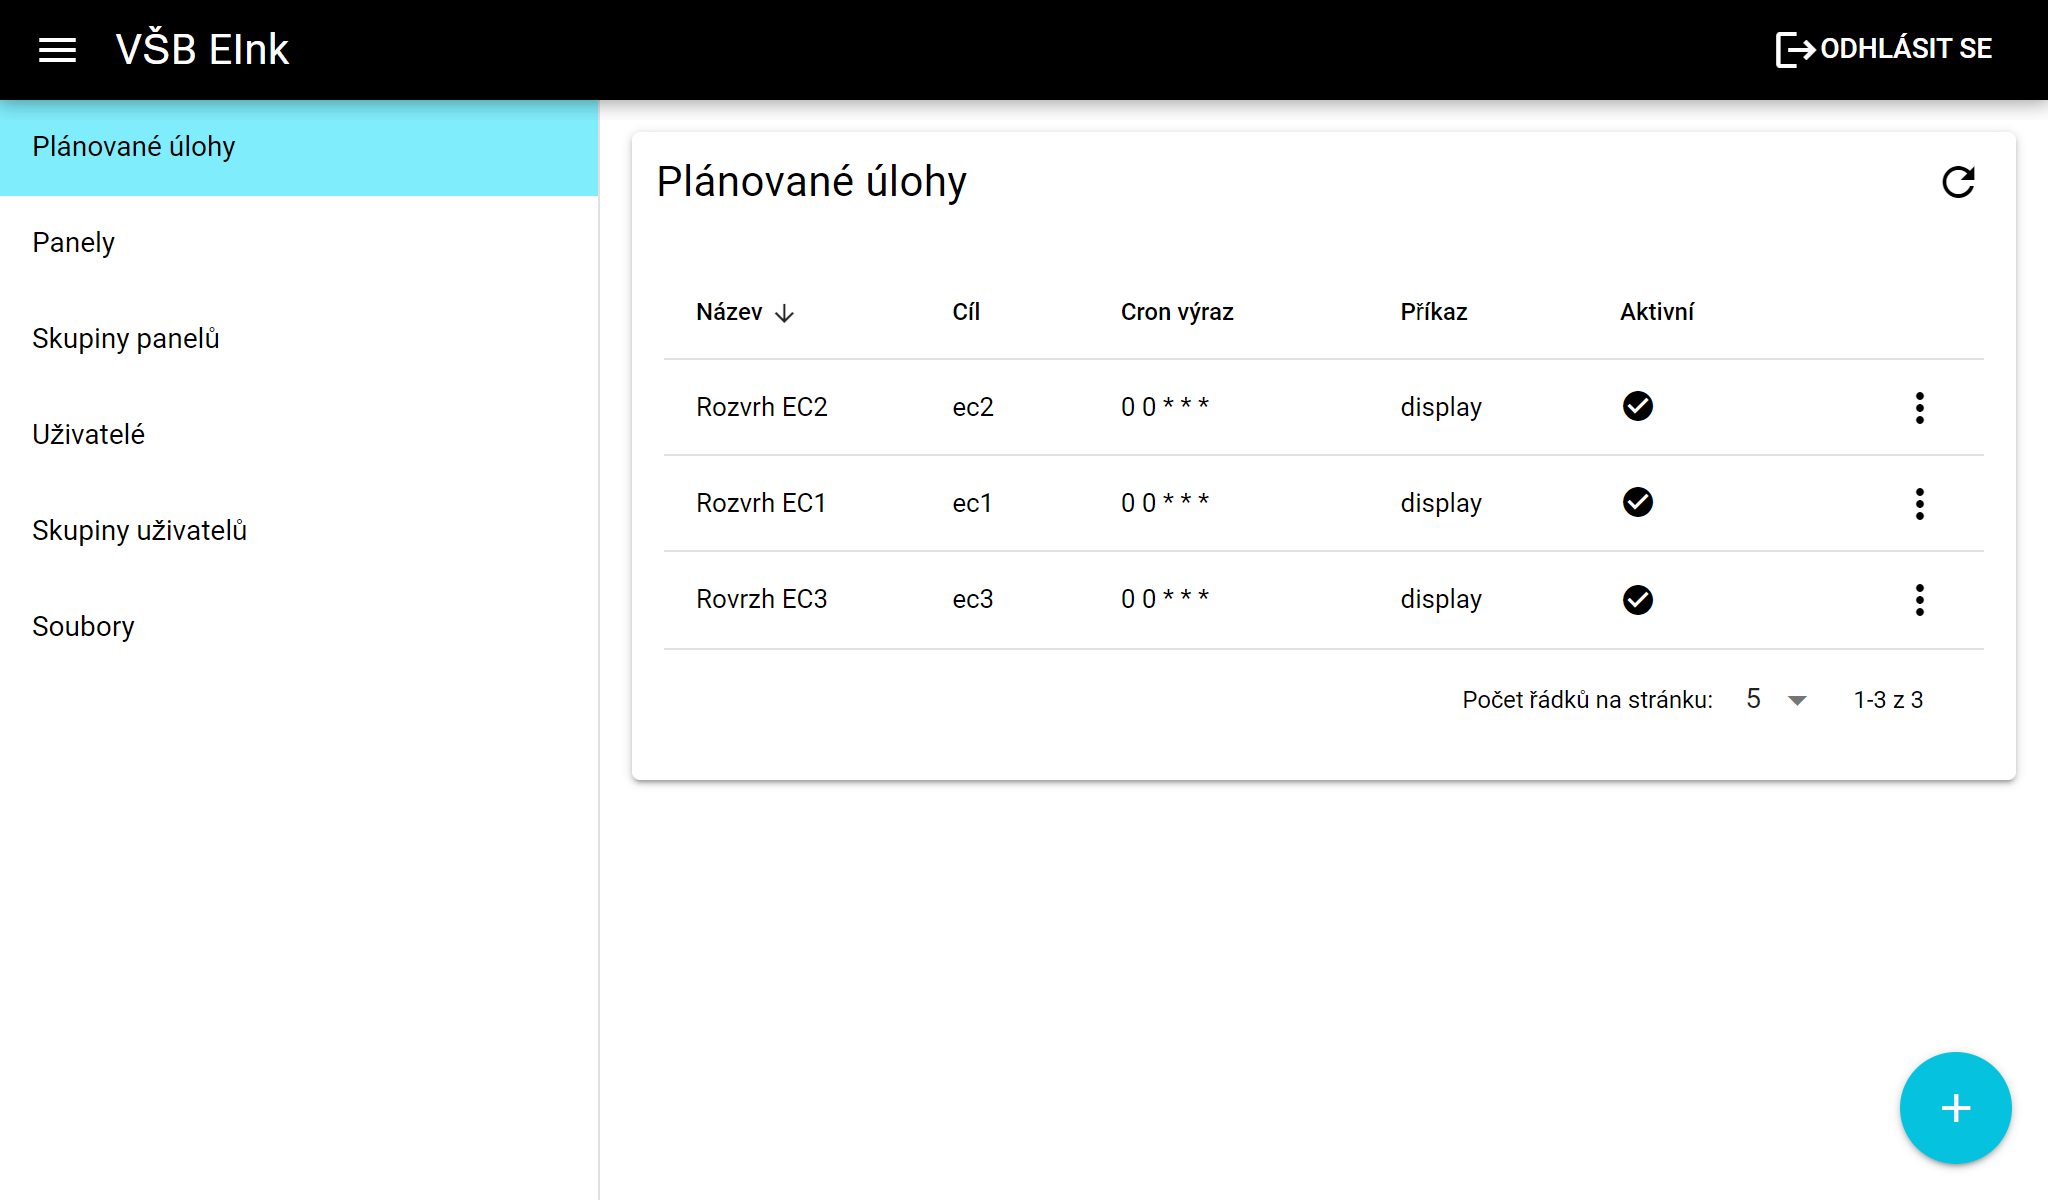
\includegraphics[width=0.70\textwidth]{Obrazky/aplikace/eink.a1314.cz_schedules.png}
    }
    \subfloat[Obrazovka plánovaných úkolů (Pixel 7)\label{fig:eink-schedules-pixel7-view}]{
        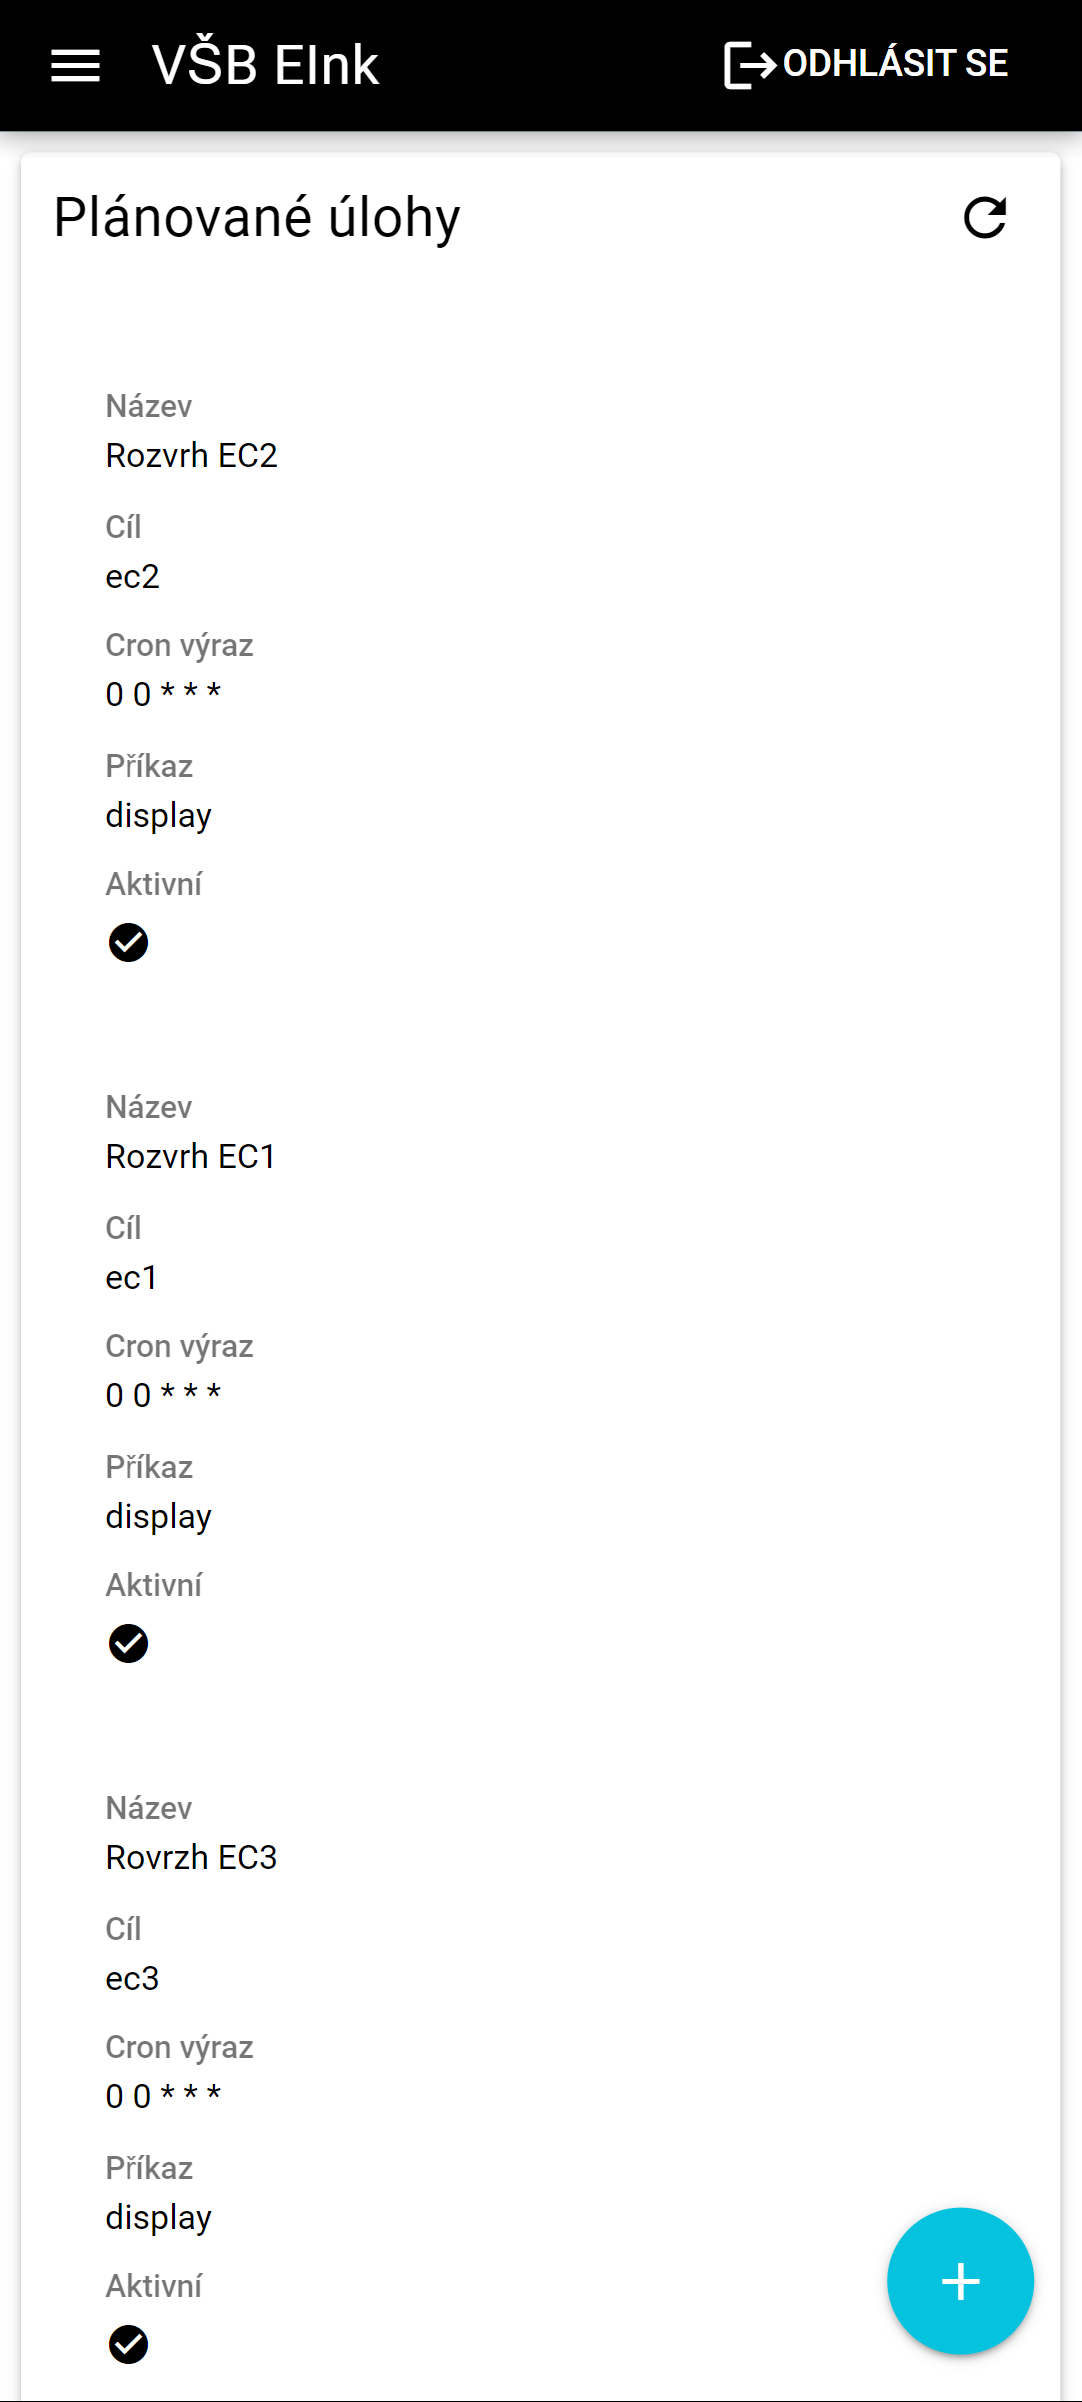
\includegraphics[width=0.28\textwidth]{Obrazky/aplikace/eink.a1314.cz_schedules_pixel7.png}
    }
    \caption{Srovnání obrazovek plánovaných úkolů na různých zařízeních}
	\label{fig:responsive-schedules}
\end{figure}


\chapter{Sestavení a nasazení}

\section{Firmware panelu}
\subsection{Sestavení}
K sestavení projektu je potřeba mít na počítači nainstalované prostředí \lstinline|esp-idf v5.0| a verzovací nástroj \lstinline|git|.

\begin{enumerate}
    \item naklonování projektu včetně submodulů \\ \lstinline{git clone --recurse-submodules git@github.com:vsb-eink/vsb-eink-panel.git}
    \item načtení prostředí \lstinline|esp-idf| \\ \lstinline{. "$IDF_PATH/export.sh"}
    \item vytvoření vlastního podpisového klíče \\ \lstinline|espsecure.py generate_signing_key certs/secure_boot_signing_key.pem|
    \item sestavení projektu \\ \lstinline|idf.py build|
\end{enumerate}

\subsubsection*{GitHub Actions}
Pro účely automatizace a zajištění opakovatelnosti sestavení, je v repozitáři \lstinline|vsb-eink-panel| zajištěno sestavování pomocí služby GitHub Actions\cite{FeaturesGitHubActions2024}. Ta je součástí sítě GitHub a je určena k použití pro automatizované sestavování a testování softwaru přímo z prostředí GitHub. Umožňuje uživatelům definovat pracovní postupy, které reagují na různé události v repozitáři, jako jsou push události, pull requesty nebo dokonce plánované události. Tyto pracovní postupy jsou popsány pomocí konfiguračních souborů ve formátu YAML a mohou být konfigurovány tak, aby spouštěly různé operace jako kompilaci kódu, spuštění testů, nebo dokonce nasazení aplikací \cite{UnderstandingGitHubActions}.

Definice procesu je uložena v souboru \lstinline|.github/workflows/build.yml|. Sestavení je spuštěno při každé úpravě soubory \lstinline|version.txt| v kořeni repozitáře, případně lze vynutit ručně.

\begin{enumerate}
    \item projekt je naklonován
    \item verze prostředí ESP-IDF je načtena ze souboru \lstinline|dependendencies.lock|
    \item verze projektu je načtena ze souboru \lstinline|version.txt|
    \item podpisový klíč, bezpečně uložený v nastavení projektu jako GitHub Repository Secret\cite{UsingSecretsGitHub}, je zapsán do souboru \lstinline|certs/secure_boot_signing_key.pem|
    \item projekt se sestaven pomocí funkce \lstinline|espressif/esp-idf-ci-action|
    \item je publikováno nové vydání firmwaru v sekci Releases pod verzí projektu ze souboru \lstinline|version.txt|
\end{enumerate}

\subsection{Nasazení}
Při vývoji nebo sestavování na vlastním stroji je nahrání firmwaru nejjednodušší pomocí příkazu \lstinline|idf.py flash|. Ten projekt sestaví a automaticky nahraje do panelu připojeného přes USB k počítači.

Pro nahrání oficiálního vydání firmwaru, je nutné stáhnout si lokálně soubory \lstinline|bootloader.bin|, \lstinline|partition-table.bin|, \lstinline|ota_data_initial.bin| a \lstinline|vsb-eink-panel.bin| ze sekce Releases repozitáře. Ty lze poté do zařízení nahrát pomocí příkazu \lstinline|esptool.py write_flash| (ukázka \ref{src:panel-firmware-flash}).

\begin{lstlisting}[label=src:panel-firmware-flash, caption={Nahrání oficiálního firmwaru do panelu}]
esptool.py -p (PORT) -b 460800 --before default_reset --after hard_reset --chip esp32  write_flash --flash_mode dio --flash_size 4MB --flash_freq 40m 0x1000 bootloader.bin 0x8000 partition-table.bin 0xd000 ota_data_initial.bin 0x10000 vsb-eink-panel.bin
\end{lstlisting}

Konfigurace panelu je popsána v sekci \ref{konfigurace-panelu}. Připravený konfigurační soubor CSV je poté nutné nahrát do zařízení příkazem \lstinline|python scripts/provision_panel.py --flash path/to/config.csv|.

Aktualizace panelů jsou možné na dálku předáním odkazu na soubor oficiálního vydání \lstinline|vsb-eink-panel.bin| skrze MQTT topik \lstinline|vsb-eink/{panel_id}/firmware/update/set|.

\section{Služby serveru a aplikace}
\subsection{Sestavení}
K sestavení projektu je potřeba Node.js 21+ a balíčkový manažer PNPM. Příkazem \lstinline|pnpm -r run build| je možné sestavit všechny komponenty projektu. PNPM při tom volá npm skript \lstinline|build| postupně podle závislostí všech balíčků.

\begin{enumerate}
    \item naklonování projektu \\ \lstinline{git clone git@github.com:vsb-eink/vsb-eink-services.git}
    \item instalace závislostí \\ \lstinline{pnpm install}
    \item vygenerování databázových a HTTP klientů \\ \lstinline{pnpm -r run generate}
    \item sestavení všech komponent projektu \\ \lstinline{pnpm -r build}
    \item sestavené soubory jsou poté uloženy v adresářích \lstinline|dist/| jednotlivých komponent 
\end{enumerate}

\subsection{Nasazení}
Pro účely nasazení je každá služba zabalena do Docker kontejneru. Jde o platformu umožňující zabalení a spuštění softwaru uvnitř izolovaného prostředí, které s hostujícím systémem sdílí pouze systémové jádro. Pro tvorbu vlastních obrazů kontejnerů je použit soubor Dockerfile popisující jednotlivé kroky stavby. Ve většině případů platí, že pokud program funguje v kontejneru na jednom počítači, měl by fungovat bez úprav i na jakémkoliv jiném počítači s nainstalovaným Dockerem bez ohledu na operační systém a verze knihoven. Navíc, protože je kontejner izolovaný od systému, nabízí vyšší míru bezpečnosti oproti programům spuštěným napřímo. Technologie, na které jsou kontejnery postaveny, jsou specifické pro Linuxové jádro \cite{DockerOverview0200}. 

Všechny komponenty sdílejí stejný Dockerfile umístěný v kořeni repozitáře. Pro efektivní sestavení jednotlivých kontejnerových obrazů je použit tzv. Multi-stage build. Jde o rozdělení Dockerfilu do sekcí, které mohou používat různá prostředí uvnitř stejného kontextu. Praktickým příkladem je například kontejner C++ programu. V jedné sekci lze nainstalovat balíčky kompilátorů a hlaviček a sestavit program do spustitelného souboru. Ve druhé sekci stačí nainstalovat pouze balíčky potřebné ke spuštění programu a sestavený soubor programu zkopírovat z první sekce. Přínosem je snížení velikosti výsledného obrazu \cite{MultistageBuilds0100}. Každá komponenta má svou vlastní sekci pro sestavení a běh. Při sestavování pomocí příkazu \lstinline|docker build| je komponenta selektována názvem své běhové sekce pomocí argumentu \lstinline|--target|.

Pro služby serveru jsem vytvořil virtuální stroj hostovaný na vlastním serveru uvnitř školní sítě. Pro jednotnou správu kontejnerů jsem použil nástroj Docker Compose a připravil soubor \lstinline|docker-compose.yml|, který popisuje a konfiguruje všechny služby systému. Kromě komunikace mezi službou Facade, webovou aplikací a prohlížečem, probíhá veškerá komunikace mezi službami po interní síti vytvořené v rámci spuštěné instance \lstinline|docker-compose.yml|. 

\subsubsection{Kontejner aplikace}
Aplikace, jakožto sada statických webových souborů, nemůže ,,běžet" samostatně. Potřebuje webový server, který soubory bude hostovat. Kontejnerizována je tedy nad obrazem kontejneru serveru Nginx, do které jsou soubory aplikace nakopírovány do výchozí sdílené složky \lstinline|/usr/share/nginx/html|. Aby výsledný kontejner bylo možné konfigurovat pomocí proměnných prostředí, stejně jako jiné kontejnery, je použit nástroj Import-meta-env. Ten při kompilaci aplikace upraví importy proměnných z objektu \lstinline|import.meta.env| tak, aby odkazovaly na proměnné na globálním objektu \lstinline|globalThis.import_meta_env|. Objekt je deklarován v souboru \lstinline|index.html| tak, aby ho bylo možné jednoduše textově nahradit. Pro zajištění, že jsou nejsou předány citlivé proměnné, jsou nahrazeny pouze proměnné z referenčního souboru \lstinline|.env|. Před spuštěním kontejneru je zavolán příkaz \lstinline|import-meta-env --disposable --example /opt/env/.env.example --path /usr/share/nginx/html/index.html|, který v HTML souboru nahradí instance proměnných prostředí zmíněných v \lstinline|.env.example| hodnotami proměnných v běhovém prostředí.

\subsubsection{Automatizace sestavení}
Podobně jako u panelu je použita služba GitHub Actions. Automat spouští sestavení při příchozím GIT tagu. Podle tagu spustí sestavení obrazů kontejneru služby či aplikace. Po sestavení jsou publikovány veřejně v registru GitHub Packages.

\begin{enumerate}
    \item je spuštěn proces pro každou komponentu
    \item procesy nevybrané TAGem jsou ukončeny
    \item projekt je naklonován
    \item proces se přihlásí ke GitHub Packages
    \item jsou extrahovány metadata z příchozího commitu pomocí \lstinline|docker/metadata-action|
    \item obraz kontejneru je sestaven a publikován funkcí \lstinline|docker/build-push-action|
\end{enumerate}

Na serveru je nasazena služba Watchtower\cite{ContainrrrWatchtower2024}, která automaticky hlídá dostupné aktualizace všech běžících kontejnerů. Pokud se vyskytne nová verze kompatibilní s aktuální verzí, kontejner je automaticky zastaven a nahrazen novou verzí. Po sestavení nových obrazů tedy stačí jen počkat a služby na serveru se aktualizují samy bez nutného zásahu správce. Upozornění o aktualizaci je zasláno skrze službu ntfy.sh\cite{NtfyShPush}.

\chapter{Závěr}

V rámci této diplomové práce byl vyvinut systém pro správu informačního panelu s využitím modulu e-ink displeje Inkplate 10. Cílem bylo vytvořit program pro e-ink displej, který umožní zobrazování různých informací, jako je rozvrh místnosti, obrázky, jednoduché animace a další, a to prostřednictvím spojení s nadřazeným systémem přes síť Wi-Fi.

V rámci práce je stručně popsán použitý hardware. Dále je popsán stav oficiálně dostupných knihoven podporujících panely Inkplate. Při vývoji bylo zjištěno, že zvolená knihovna Inkplate ESP-IDF obsahuje určité nedostatky. Byl vytvořen fork této knihovny a ten byl upraven tak, aby ji bylo možné dále používat.

Byl vytvořen program, který umožňuje modulu e-ink displeje připojení k nadřazenému systému přes Wi-Fi s využitím MQTT protokolu. Program je schopen zobrazovat bitmapové obrázky a pomocí MQTT zpráv jej lze konfigurovat.

Pro účely uživatelského ovládání byla vytvořena sada serverových služeb a webové rozhraní. Systém umožňuje centrální správu více e-ink displejů a definování obsahu, který se na nich zobrazuje. Tento systém je přístupný skrze webové rozhraní, které podporuje autentizaci a umožňuje uživatelům přizpůsobit zobrazení na konkrétních displejích.

Systém byl nasazen na panelech u přednáškových místností EC1, EC2 a EC3. Tyto panely byly v nepřetržitém provozu po dobu 6 měsíců a většinu této doby zobrazovaly informace o počasí, čase a novinkách školy s aktualizací každou minutu.

V rámci testování se ukázaly nedostatky v efektivitě některých služeb, zejména služby Renderer, zodpovědné za zpracování webových dokumentů pro zobrazení na e-ink panelech. Tato část systému by měla být v budoucnu optimalizována tak, aby byla zajištěna kompatibilita s komplexními webovými dokumenty a včasného zobrazení obsahu. Případně musí být tato služba provozována na výkonnějším serveru, než který jsem měl k dispozici.

Osobně plánuji pokračovat ve vývoji systému i nadále. Panel Inkplate 10 si hodlám pořídit pro soukromé účely a chci jej využít jako obrazovku pro zobrazení dat služby Home Assistant\cite{HomeassistantCoreHouse_with_garden}.

\newpage
Projekt je vyvíjen otevřeně na platformě GitHub pod organizací \href{https://github.com/vsb-eink/}{VŠB-EInk}.
\begin{table}[h]
    \begin{tabular}{ll}
        Monorepozitář serveru + aplikace & \url{https://github.com/vsb-eink/vsb-eink-services} \\
        Firmware panelu & \url{https://github.com/vsb-eink/vsb-eink-panel} \\
    \end{tabular}
\end{table}

% Seznam literatury
\printbibliography[title={Literatura}, heading=bibintoc]

% Prilohy
\appendix
\input{Prilohy/Priloha1}
\input{Prilohy/Priloha2}

\end{document}
